\documentclass[a0,portrait]{a0poster}

\usepackage{palatino}
\usepackage{mathpazo}

\usepackage{multicol}
\columnsep=100pt
\columnseprule=3pt

\usepackage[svgnames]{xcolor}

\usepackage{graphicx}
\graphicspath{{figs/}}
\usepackage{booktabs}
\usepackage[font=small,labelfont=bf]{caption}
\usepackage{amsmath, amsthm, amssymb}
\usepackage{wrapfig}
\usepackage{hhline}

\usepackage{nicefrac}
\usepackage{bm}
\usepackage{siunitx}
\usepackage{tikz}
\usepackage{pgfplots}
\usetikzlibrary{positioning}
\usetikzlibrary{arrows.meta}
\usepgfplotslibrary{groupplots}

\definecolor{darkblue}{HTML}{00688B}
\definecolor{darkgreen}{HTML}{6E8B3D}
\definecolor{cadet}{HTML}{DAE1FF}
\definecolor{salmon}{HTML}{FFB08A}

\begin{document}

\begin{minipage}[b]{1.0\linewidth}
  \veryHuge \color{NavyBlue}
  \textbf{\noindent Fast divergence-conforming reduced basis methods \\ for stationary and transient flow problems}
  \color{Black}\\
\end{minipage}
\begin{minipage}[b]{0.7\linewidth}
  \huge \textbf{E.~Fonn, H.~v.~Brummelen, T.~Kvamsdal, A.~Rasheed}\\[0.5cm]
  \huge SINTEF Digital\\[0.4cm]
  \Large eivind.fonn@sintef.no --- +47 41 44 98 89\\
\end{minipage}
%
\begin{minipage}[b]{0.25\linewidth}
  \includegraphics[width=20cm]{common/sintef}\\
\end{minipage}

\vspace{1cm}

\begin{multicols}{2}

\color{DarkSlateGray}
\Large

\begin{wrapfigure}{l}{0.20\textwidth}
  \begin{tikzpicture}[scale=15]
    \draw[very thick, ->] (0,0) -- (1,0);
    \draw[very thick, ->] (0,0) -- (0,1);
    \node[anchor=south west] at (0,0) {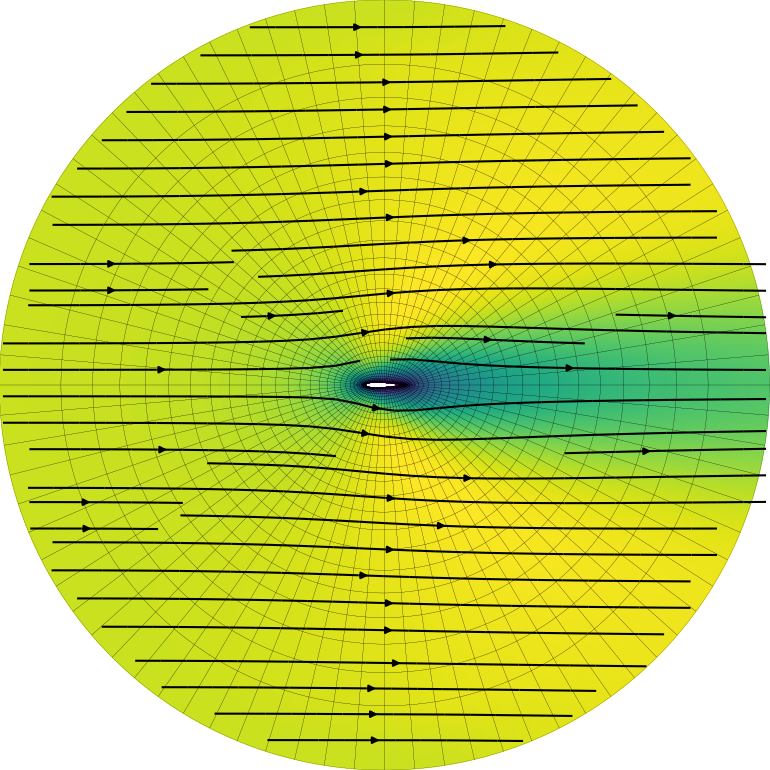
\includegraphics[width=68mm]{figs/full-lo-lo}};
    \node[anchor=south east] at (1,0) {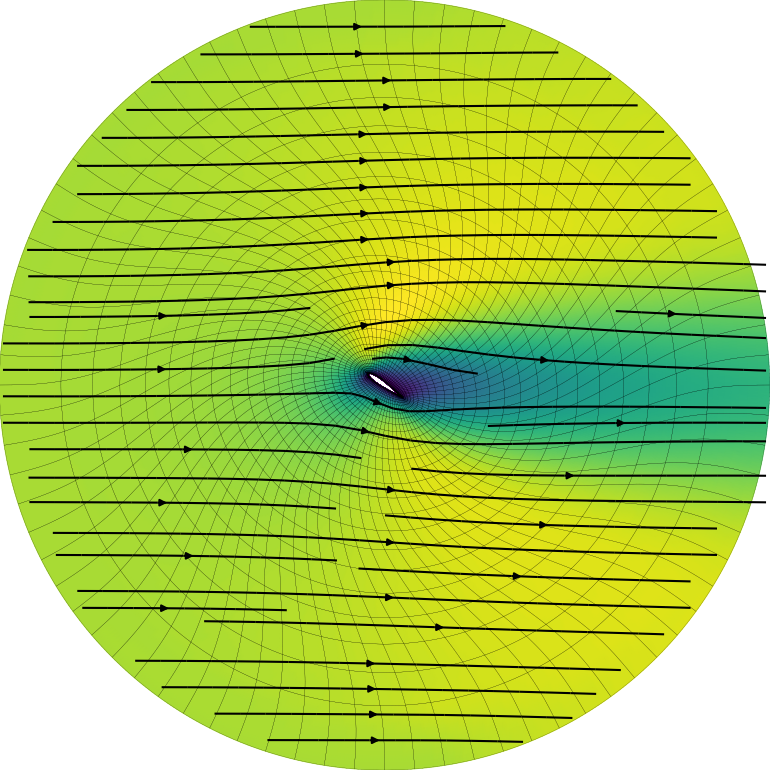
\includegraphics[width=68mm]{figs/full-hi-lo}};
    \node[anchor=north east] at (1,1) {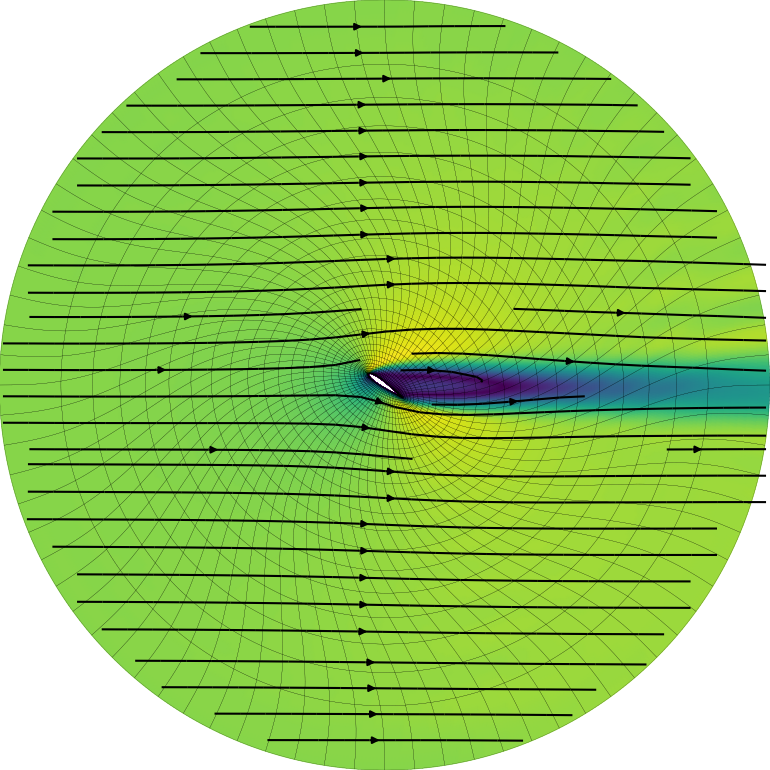
\includegraphics[width=68mm]{figs/full-hi-hi}};
    \node[anchor=north west] at (0,1) {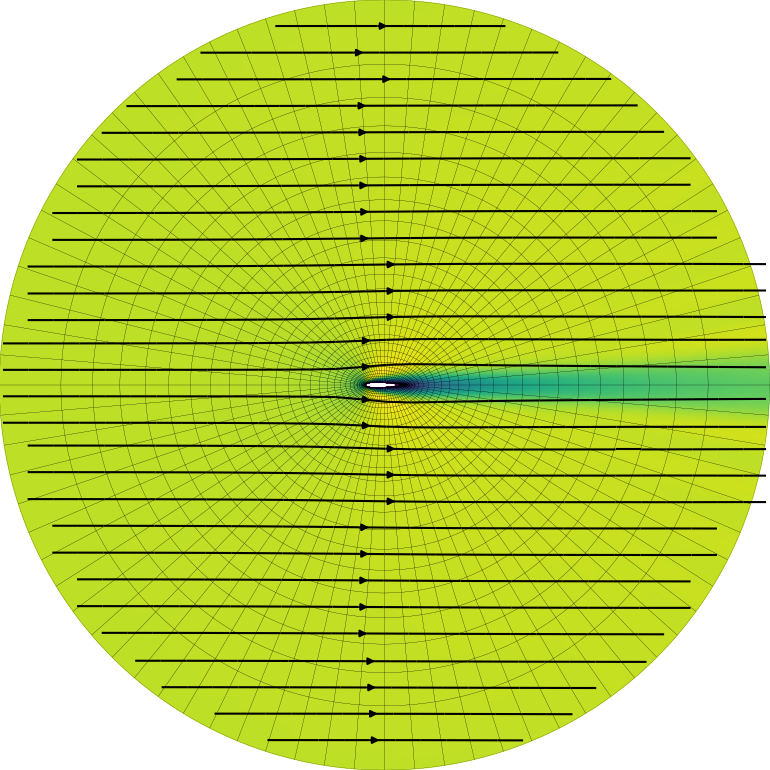
\includegraphics[width=68mm]{figs/full-lo-hi}};
    \node[anchor=north] at (0.5,0) {Angle of attack ($\varphi$)};
    \node[anchor=south, rotate=90] at (0,0.5) {Airspeed ($u_\infty$)};
  \end{tikzpicture}
\end{wrapfigure}

\noindent \textbf{Problem:} Repeated solutions of parametrized
problems (left) can be extremely demanding, each query involving up to
$10^6$--$10^9$ degrees of freedom and hours or days of computational
time.

\noindent \textbf{Solution:} Reduced Order Modelling (ROM) via Reduced
Basis Methods (RBM) offers solutions with dramatic speedups and
respectable accuracy.

\begin{center}
  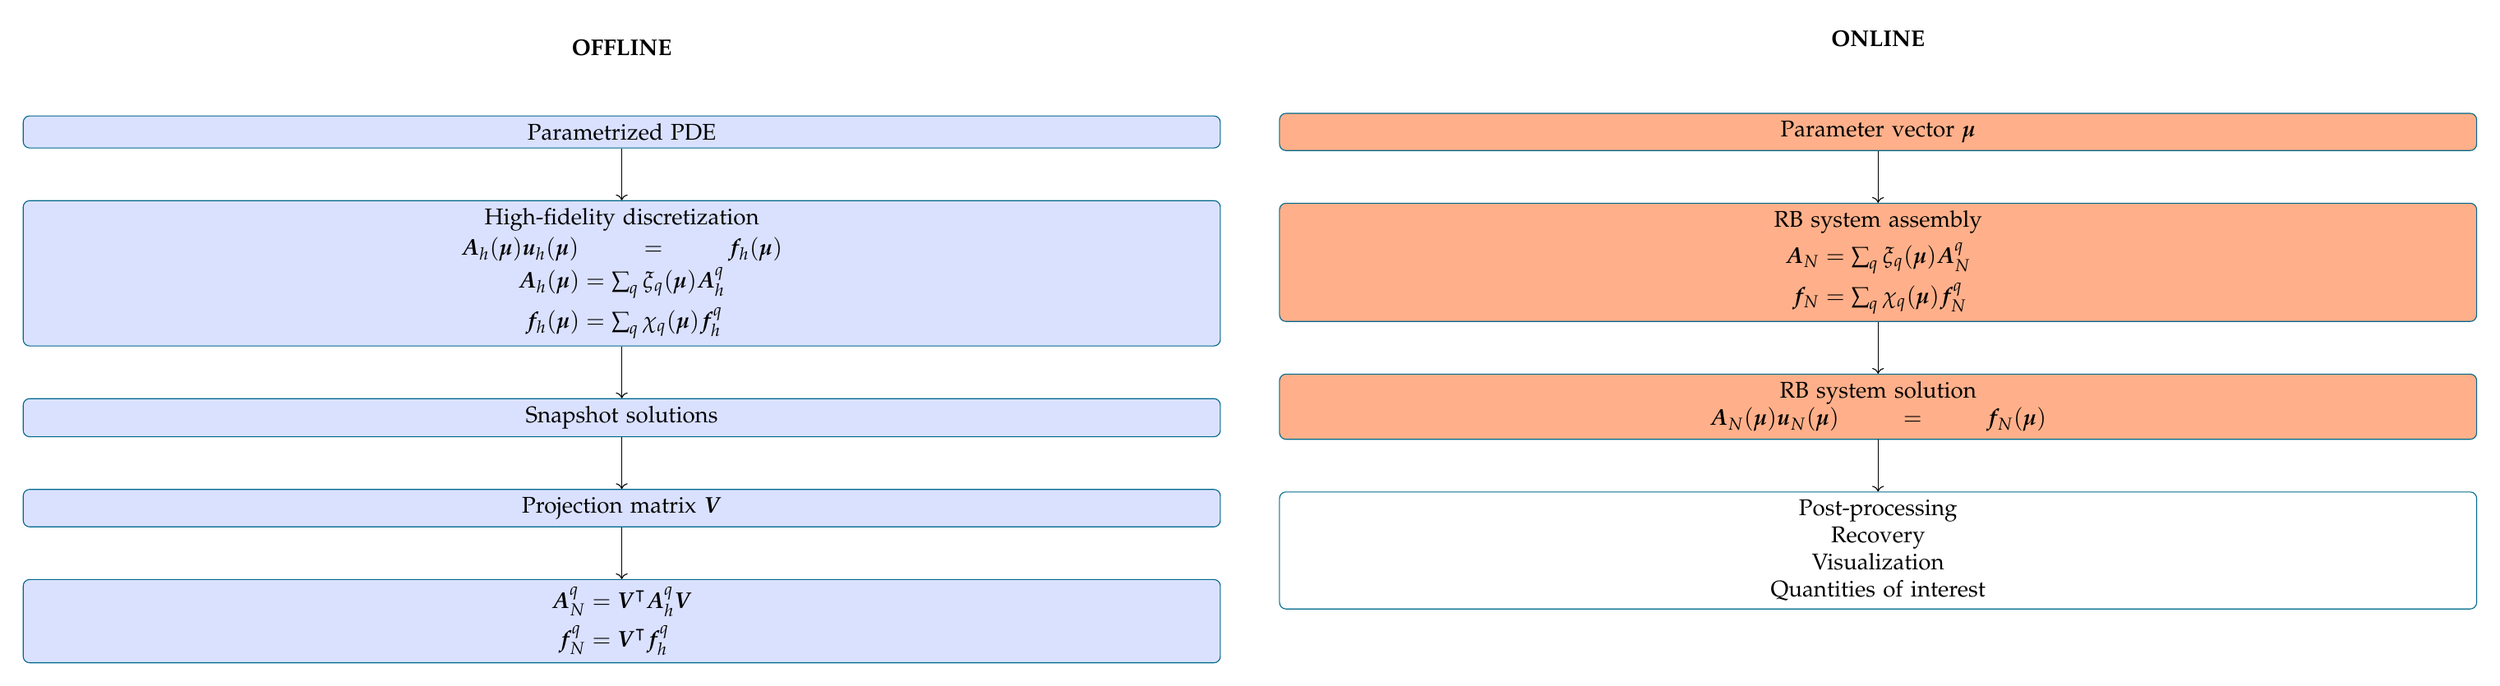
\begin{tikzpicture}[
    block/.style={
      minimum width=185mm,
      text width=180mm,
      align=center,
      rounded corners=1mm,
    },
    offline/.style={
      block,
      draw=darkblue,
      fill=cadet,
    },
    online/.style={
      block,
      draw=darkblue,
      fill=salmon,
    },
    clear/.style={
      block,
      draw=darkblue,
    },
    ]
    \node[] (offline) {\textbf{OFFLINE}};
    \node[offline, below=8mm of offline] (pde) {Parametrized PDE};
    \node[offline, below=8mm of pde] (hifi) {
      High-fidelity discretization \\[0.5mm]
      $\bm A_h(\bm \mu) \bm u_h(\bm \mu) = \bm f_h(\bm \mu)$ \\[0.5mm]
      $\begin{aligned}
        \bm A_h(\bm \mu) &= \textstyle \sum_q \xi_q(\bm \mu) \bm A_h^q \\
        \bm f_h(\bm \mu) &= \textstyle \sum_q \chi_q(\bm \mu) \bm f_h^q
      \end{aligned}$
    };
    \node[offline, below=8mm of hifi] (snaps) {
      Snapshot solutions
    };
    \node[offline, below=8mm of snaps] (mx) {
      Projection matrix $\bm V$
    };
    \node[offline, below=8mm of mx] (proj) {
      $\begin{aligned}
        \bm A^q_N &= \bm V^\intercal \bm A_h^q \bm V \\
        \bm f^q_N &= \bm V^\intercal \bm f_h^q
      \end{aligned}$
    };
    \node[online, right=9mm of pde] (mu) {Parameter vector $\bm \mu$};
    \node[above=9mm of mu] (online) {\textbf{ONLINE}};
    \node[online, below=8mm of mu] (asm) {
      RB system assembly \\[1.0mm]
      $\begin{aligned}
        \bm A_N &= \textstyle \sum_q \xi_q(\bm \mu) \bm A^q_N \\
        \bm f_N &= \textstyle \sum_q \chi_q(\bm \mu) \bm f^q_N
      \end{aligned}$
    };
    \node[online, below=8mm of asm] (sol) {
      RB system solution \\[0.0mm]
      $\bm A_N(\bm \mu) \bm u_N(\bm \mu) = \bm f_N(\bm \mu)$
    };
    \node[clear, below=8mm of sol] (err) {
      Post-processing \\ Recovery \\ Visualization \\ Quantities of interest
    };

    \draw[->] (pde.south) -- (hifi.north);
    \draw[->] (hifi.south) -- (snaps.north);
    \draw[->] (snaps.south) -- (mx.north);
    \draw[->] (mx.south) -- (proj.north);
    \draw[->] (mu.south) -- (asm.north);
    \draw[->] (asm.south) -- (sol.north);
    \draw[->] (sol.south) -- (err.north);
  \end{tikzpicture}
\end{center}

\noindent \textbf{Stationary:} Navier-Stokes flow around a NACA0015 airfoil with
chord length of $\SI{1}{\meter}$, parametrized by inflow velocity
$u_\infty \in [\SI{1}{\meter/\second}, \SI{20}{\meter/\second}]$ and
angle of attack $\varphi \in [\SI{-35}{\degree},
\SI{35}{\degree}]$. Snapshots were evaluated on the $15 \times 15$
Gauss points on the parameter domain and reduced models created with
$N=10,20,\ldots,50$ DoFs.

\vspace{1cm}

\noindent \textbf{Transient:} Navier-Stokes flow around a cylinder
with diameter $\SI{1}{\meter}$, inflow velocity
$\SI{1}{\meter/\second}$ and $\text{Re}=100$. This system has two
\emph{stages}: a transient stage influenced by the initial velocity
field and a stable, perpetual vortex shedding stage. Snapshots were
evaluated \emph{only} in the vortex shedding stage, and reduced models
created with $N=5,10,15,20$ DoFs.

\begin{center}
  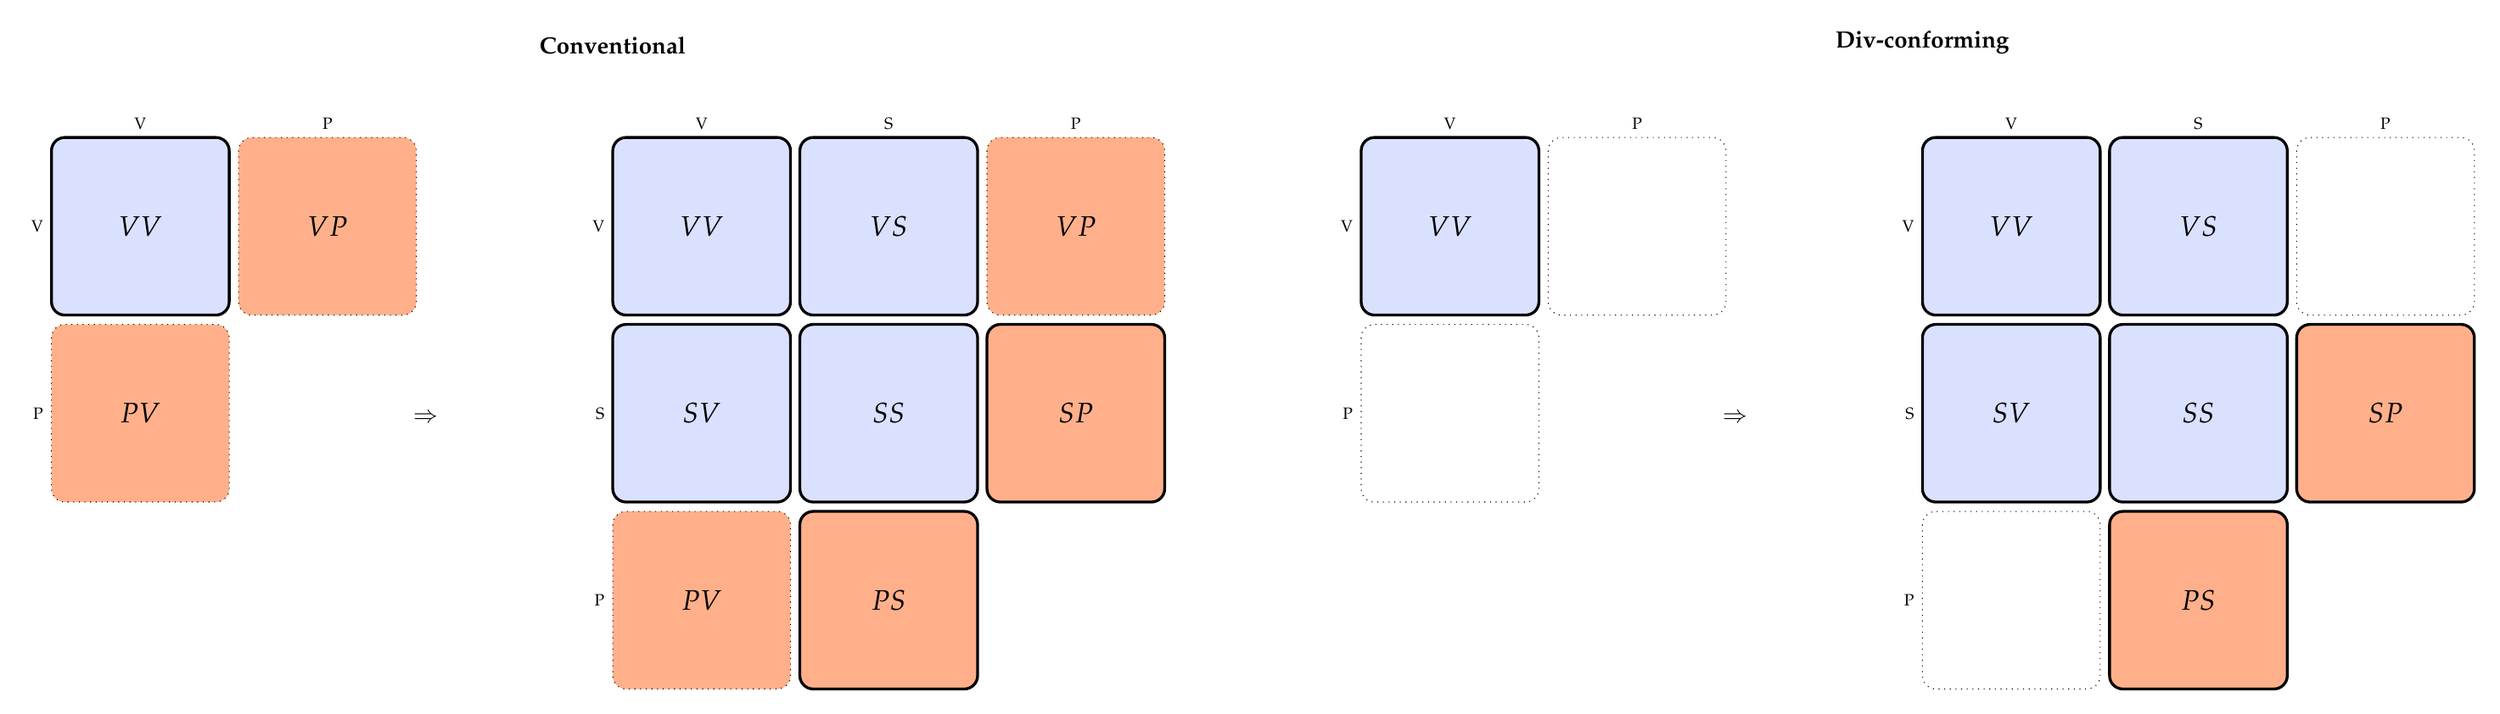
\begin{tikzpicture}[scale=2.8]
    \node[anchor=south] at (3,0.4) {\textbf{Conventional}};

    \node[anchor=south] at (0.475,0) {\scriptsize V};
    \node[anchor=south] at (1.475,0) {\scriptsize P};
    \node[anchor=east] at (0,-0.475) {\scriptsize V};
    \node[anchor=east] at (0,-1.475) {\scriptsize P};

    \fill[cadet, draw=black, very thick, rounded corners=2mm] (0,0) rectangle (0.95,-0.95);
    \fill[salmon, draw=black, dotted, rounded corners=2mm] (1,0) rectangle (1.95,-0.95);
    \fill[salmon, draw=black, dotted, rounded corners=2mm] (0,-1) rectangle (0.95,-1.95);
    \node at (0.475,-0.475) {\large $VV$};
    \node at (1.475,-0.475) {\large $VP$};
    \node at (0.475,-1.475) {\large $PV$};

    \node at (2.0,-1.5) {$\Rightarrow$};

    \node[anchor=south] at (3.475,0) {\scriptsize V};
    \node[anchor=south] at (4.475,0) {\scriptsize S};
    \node[anchor=south] at (5.475,0) {\scriptsize P};
    \node[anchor=east] at (3,-0.475) {\scriptsize V};
    \node[anchor=east] at (3,-1.475) {\scriptsize S};
    \node[anchor=east] at (3,-2.475) {\scriptsize P};

    \fill[cadet, draw=black, very thick, rounded corners=2mm] (3,0) rectangle (3.95,-0.95);
    \fill[cadet, draw=black, very thick, rounded corners=2mm] (4,0) rectangle (4.95,-0.95);
    \fill[cadet, draw=black, very thick, rounded corners=2mm] (3,-1) rectangle (3.95,-1.95);
    \fill[cadet, draw=black, very thick, rounded corners=2mm] (4,-1) rectangle (4.95,-1.95);
    \fill[salmon, draw=black, dotted, rounded corners=2mm] (5,0) rectangle (5.95,-0.95);
    \fill[salmon, draw=black, dotted, rounded corners=2mm] (3,-2) rectangle (3.95,-2.95);
    \fill[salmon, draw=black, very thick, rounded corners=2mm] (5,-1) rectangle (5.95,-1.95);
    \fill[salmon, draw=black, very thick, rounded corners=2mm] (4,-2) rectangle (4.95,-2.95);
    \node at (3.475,-0.475) {\large $VV$};
    \node at (4.475,-0.475) {\large $VS$};
    \node at (5.475,-0.475) {\large $VP$};
    \node at (3.475,-1.475) {\large $SV$};
    \node at (4.475,-1.475) {\large $SS$};
    \node at (5.475,-1.475) {\large $SP$};
    \node at (3.475,-2.475) {\large $PV$};
    \node at (4.475,-2.475) {\large $PS$};

    \node[anchor=south] at (10,0.4) {\textbf{Div-conforming}};

    \node[anchor=south] at (7.475,0) {\scriptsize V};
    \node[anchor=south] at (8.475,0) {\scriptsize P};
    \node[anchor=east] at (7,-0.475) {\scriptsize V};
    \node[anchor=east] at (7,-1.475) {\scriptsize P};

    \fill[cadet, draw=black, very thick, rounded corners=2mm] (7,-0) rectangle (7.95,-0.95);
    \draw[black, dotted, rounded corners=2mm] (8,-0) rectangle (8.95,-0.95);
    \draw[black, dotted, rounded corners=2mm] (7,-1) rectangle (7.95,-1.95);
    \node at (7.475,-0.475) {\large $VV$};

    \node at (9.0,-1.5) {$\Rightarrow$};

    \node[anchor=south] at (10.475,0) {\scriptsize V};
    \node[anchor=south] at (11.475,0) {\scriptsize S};
    \node[anchor=south] at (12.475,0) {\scriptsize P};
    \node[anchor=east] at (10,-0.475) {\scriptsize V};
    \node[anchor=east] at (10,-1.475) {\scriptsize S};
    \node[anchor=east] at (10,-2.475) {\scriptsize P};

    \fill[cadet, draw=black, very thick, rounded corners=2mm] (10,0) rectangle (10.95,-0.95);
    \fill[cadet, draw=black, very thick, rounded corners=2mm] (11,0) rectangle (11.95,-0.95);
    \fill[cadet, draw=black, very thick, rounded corners=2mm] (10,-1) rectangle (10.95,-1.95);
    \fill[cadet, draw=black, very thick, rounded corners=2mm] (11,-1) rectangle (11.95,-1.95);
    \draw[black, dotted, rounded corners=2mm] (12,0) rectangle (12.95,-0.95);
    \draw[black, dotted, rounded corners=2mm] (10,-2) rectangle (10.95,-2.95);
    \fill[salmon, draw=black, very thick, rounded corners=2mm] (12,-1) rectangle (12.95,-1.95);
    \fill[salmon, draw=black, very thick, rounded corners=2mm] (11,-2) rectangle (11.95,-2.95);
    \node at (10.475,-0.475) {\large $VV$};
    \node at (11.475,-0.475) {\large $VS$};
    \node at (10.475,-1.475) {\large $SV$};
    \node at (11.475,-1.475) {\large $SS$};
    \node at (12.475,-1.475) {\large $SP$};
    \node at (11.475,-2.475) {\large $PS$};
  \end{tikzpicture}
\end{center}

\noindent \textbf{Div-conforming RBMs are faster:} The reduced system
matrix (size $2N$) will usually have a rank-deficient
velocity-pressure block (denoted VP). Enriching the velocity space
with so-called \emph{supremizers} (denoted S) ensures a full-rank
system matrix with size $3N$. A div-conforming method instead produces
a fully divergence-free basis, so the VP block vanishes. This yields a
block-triangular system, solvable as two size-$N$ systems instead of
one size-$3N$ system.

\section*{\LARGE Acknowledgements}

The authors acknowledge the financial support from the Norwegian
Research Council and the industrial partners of OPWIND: Operational
Control for Wind Power Plants (Grant No.: 268044/E20).

\begin{center}
  \textbf{Mean solver time usage}
  \bgroup\def\arraystretch{1.3}
  \setlength\tabcolsep{5mm}
  \begin{tabular}{r!{\color{black!20!white}\vrule}r!{\color{black!20!white}\vrule}r!{\color{black!20!white}\vrule}r!{\color{black!20!white}\vrule}r!{\color{black!20!white}\vrule}r!{\color{black!20!white}\vrule}r}
    & Hi-Fi & $N=10$ & $N=20$ & $N=30$ & $N=40$ & $N=50$ \\ \hhline{=======}
    Conventional & $\SI{104}{\second}$ & $\SI{29}{\milli\second}$ & $\SI{126}{\milli\second}$ & $\SI{503}{\milli\second}$ & $\SI{1.02}{\second}$ & $\SI{2.51}{\second}$ \\ \hline
    Conforming & $\SI{165}{\second}$ & $\SI{21}{\milli\second}$ & $\SI{54}{\milli\second}$ & $\SI{104}{\milli\second}$ & $\SI{183}{\milli\second}$ & $\SI{284}{\milli\second}$
  \end{tabular}
  \egroup
\end{center}

\vfill

\begin{center}
  \textbf{Stationary: error vs.~speed}
  \begin{tikzpicture}
    \begin{axis}[
      xlabel={Time (sec)},
      x label style={at={(axis description cs:0.67,0.02)}, anchor=north},
      ylabel={Error},
      y label style={at={(axis description cs:0.02,0.61)}, anchor=south},
      ymode=log,
      xmode=log,
      width=0.45\textwidth,
      height=0.2\textwidth,
      grid=both,
      legend style={
        at={(0.5, -0.2)},
        anchor=north,
        draw=none,
      },
      legend cell align=left,
      ]
      \addplot[blue, line width=5pt, mark=*, mark options={solid}]
      table[x index={15}, y index={4}]{data/airfoil-results-no-piola-sups-no-block.csv};
      \addplot[blue, line width=5pt, dotted, mark=o, mark options={solid}, forget plot]
      table[x index={15}, y index={8}]{data/airfoil-results-no-piola-sups-no-block.csv};
      \addplot[green, line width=5pt, mark=*, mark options={solid}]
      table[x index={11}, y index={4}]{data/airfoil-results-piola-sups-block.csv};
      \addplot[green, line width=5pt, dotted, mark=o, mark options={solid}, forget plot]
      table[x index={11}, y index={8}]{data/airfoil-results-piola-sups-block.csv};
      \addplot[cyan, line width=5pt, mark=*, mark options={solid}]
      table[x index={11}, y index={4}]{data/airfoil-results-combined.csv};
      \addplot[cyan, line width=5pt, dotted, mark=o, mark options={solid}, forget plot]
      table[x index={11}, y index={8}]{data/airfoil-results-combined.csv};
      \legend{
        {Conventional ($v,p$)},
        {Conforming pressure recovery ($v,p$)},
        {Conforming pressure reconstruction ($v,p$)},
      }
    \end{axis}
  \end{tikzpicture}
\end{center}

\begin{center}
  \textbf{Transient: drag force vs.~time}
  \begin{tikzpicture}
    \begin{axis}[
      xlabel={Time},
      ylabel={Drag force},
      xticklabels={,,},
      yticklabels={,,},
      ymin=0.5, ymax=0.7,
      xmin=2000, xmax=50000,
      restrict x to domain=2000:50000,
      scaled x ticks=false,
      width=0.45\textwidth,
      height=0.2\textwidth,
      grid=both,
      legend style={
        at={(0.5, -0.2)},
        anchor=north,
        draw=none,
        /tikz/column 2/.style={column sep=1cm},
        /tikz/column 4/.style={column sep=1cm},
        /tikz/column 6/.style={column sep=1cm},
        /tikz/column 8/.style={column sep=1cm},
      },
      legend columns=5,
      ]
      \addplot[black, very thick] table[x index={0}, y index={1}]{data/sparseforces.csv};
      \addplot[red, very thick] table[x expr={\thisrowno{0}*25}, y index={1}]{data/forces-05.csv};
      \addplot[blue, very thick] table[x expr={\thisrowno{0}*25}, y index={1}]{data/forces-10.csv};
      \addplot[magenta, very thick] table[x expr={\thisrowno{0}*25}, y index={1}]{data/forces-15.csv};
      \addplot[cyan, very thick] table[x expr={\thisrowno{0}*25}, y index={1}]{data/forces-20.csv};
      \draw[densely dotted, very thick] (axis cs:0,0.655) -- (axis cs:50000,0.655);
      \draw[densely dotted, very thick] (axis cs:0,0.649) -- (axis cs:50000,0.649);
      \legend{Hi-Fi, $N=5$, $N=10$, $N=15$, $N=20$};
    \end{axis}
  \end{tikzpicture}
\end{center}

\begin{center}
  \textbf{Transient: lift force vs.~time}
  \begin{tikzpicture}
    \begin{axis}[
      xlabel={Time},
      ylabel={Lift force},
      xticklabels={,,},
      yticklabels={,,},
      ymin=-0.14, ymax=0.14,
      xmin=0, xmax=800,
      restrict x to domain=0:800,
      scaled x ticks=false,
      width=0.45\textwidth,
      height=0.2\textwidth,
      grid=both,
      legend style={
        at={(0.5, -0.2)},
        anchor=north,
        draw=none,
        /tikz/column 2/.style={column sep=1cm},
        /tikz/column 4/.style={column sep=1cm},
        /tikz/column 6/.style={column sep=1cm},
        /tikz/column 8/.style={column sep=1cm},
      },
      legend columns=5,
      ]
      \addplot[black, thin] table[x expr={\thisrowno{0}-13500}, y index={2}]{data/forces.csv};
      \addplot[red, thin] table[x expr={\thisrowno{0}-8}, y index={2}]{data/denseforces-05.csv};
      \addplot[blue, thin] table[x expr={\thisrowno{0}+16}, y index={2}]{data/denseforces-10.csv};
      \addplot[magenta, thin] table[x expr={\thisrowno{0}-62}, y index={2}]{data/denseforces-15.csv};
      \addplot[cyan, thin] table[x expr={\thisrowno{0}-32}, y index={2}]{data/denseforces-20.csv};
      \legend{Hi-Fi, $N=5$, $N=10$, $N=15$, $N=20$};
    \end{axis}
  \end{tikzpicture}
\end{center}

\section*{\LARGE Discussion}

\begin{itemize}
\item RBMs are able to deliver results within two to three orders of
  magnitude at dramatic speedups.
\item Div-conforming RBMs can deliver higher speeds (one order of
  magnitude in present examples) by exploiting specific properties of
  velocity basis functions.
\item RBMs based only on final stage (vortex shedding) snapshots can
  still step through the transient stage without permanent loss of
  accuracy (e.g.~blowing up or crashing).
\end{itemize}

\end{multicols}

\end{document}
